%%%%%%%%%%%%%%%%%%%%% chapter.tex %%%%%%%%%%%%%%%%%%%%%%%%%%%%%%%%%
%
% sample chapter
%
% Use this file as a template for your own input.
%
%%%%%%%%%%%%%%%%%%%%%%%% Springer-Verlag %%%%%%%%%%%%%%%%%%%%%%%%%%
%\motto{Use the template \emph{chapter.tex} to style the various elements of your chapter content.}
\chapter{Geometry of Relativity}
\label{Geom} % Always give a unique label
% use \chaptermark{}
% to alter or adjust the chapter heading in the running head



\abstract{In this chapter we begin the discussion of the relation between gravity and geometry. In particular, we remark that Gravity is simply the geometry of space time, with objects following straight paths or ``geodesics" in the curved space time. For this purpose we study a few common geometries, and how we can use the notion of a Riemannian metric, or \textbf{line element}, to generalize our understanding of geometry from the Euclidean setting to spherical geometries and beyond.}

\section{Gravity and Geometry}
\label{sec:gravGeom}

As we shall soon be aware, gravity \textbf{is} geometry---it arises from the curvature of \textbf{spacetime}. The fact that all bodies fall with the same acceleration in a uniform gravitational field, independently of their composition, is one of the most accurately tested facts in physics. The most accurate such test is the comparison of the accelerations of the Earth and the Moon as they fall around the Sun. These match to within a fractional error of less than $1.5\times 10^{-13}$.

\begin{figure}[H]
    \centering
    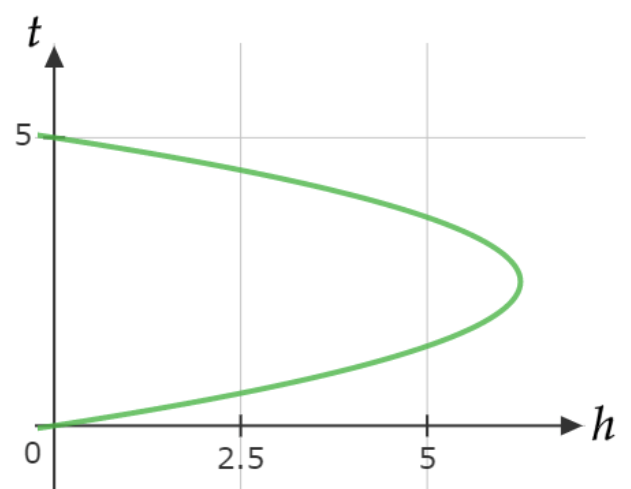
\includegraphics[scale = 0.5]{ParabolTraj.PNG}
    \caption{Space-time diagram for object thrown vertically on earth with height on the horizontal.}
    \label{fig:parabolTraj}
\end{figure}

In Einstein's general relativity, the bodies are following a straight path in the curved spacetime produced by the Earth's mass. Note that the exact same trajectory pictured above would occur for any other body with the same initial velocity and same initial position. This uniqueness property is not seen in all other fields. For instance, the motion of a body in a magnetic field depends on what kind of charge it has. Bodies with one sign of charge will be deflected one way, bodies with the opposite charge will be deflected the other, and bodies with no charge will not be deflected at all.

Einstein proposed that in the absence of other forces, bodies move on straight paths in this curved spacetime.

\section{Experiments in Geometry}
\label{sec:ExpGeom}

Geometries different from Euclid's produce different results for the sum of the interior angles of a triangle. For instance, due to the curvature of the Earth, the interior angles of a triangle on its surface would deviate from $\pi$ on the order of: $$\left|\left(\begin{array}{c} \text{sum of interior angles} \\ \text{of a triangle in radians}\end{array}\right)\right| - \pi \sim \frac{(\text{area of triangle})}{R_{\oplus}^2}\left(\frac{GM_{\oplus}}{R_{\oplus}c^2}\right)$$
where $\oplus$ denotes the Earth. 


\section{Different Geometries}
\label{sec:DiffGeom}

When we talk about straight paths in different geometries, we mean paths of shortest distance between two points, which generalized the notion of straight lines in Euclidean Geometry. In Spherical geometry these are segments of great circles (circles which cut through the origin of the sphere). Triangles on the sphere are then made of three intersecting great circles. For a spherical triangle of area $A$, $$\sum_{vertices}\left(\begin{array}{c} \text{interior} \\ \text{angle}\end{array}\right) = \pi + \frac{A}{a^2}$$
where $a$ is the radius of the sphere.

Note this implies that the sum of the interior angles of a spherical triangle is always greater than $\pi$.

With a bit of geometry, the ratio of the circumference to the radius of a circle on a sphere can be calculated to be $$\frac{C}{r} = \frac{2\pi a\sin(r/a)}{r} = 2\pi\frac{\sin(r/a)}{(r/a)}$$

In theory by surveying in three dimensions we can determine the geometry of space without needing an extra dimension. However, visualization of three dimensional geometries is in general very difficult. An example which is simpler, at least to describe, is the three-sphere. If space had such a geometry a journey in a straight line in any direction would eventuallly bring one back to the starting points. However, we can determine more detail locally. For instance, the volume inside a two-dimensional sphere of radius $r$ in such a spatial geometry is given by \begin{align*}
    V &= 4\pi a^3\left\{\frac{1}{2}\sin^{-1}(r/a)-\frac{r}{2a}\left[1-\frac{r^2}{a^2}\right]^{1/2}\right\} \\
    &\approx \frac{4\pi r^3}{3}\left[1+\left(\begin{array}{c} \text{corrections} \\ \text{of order }(r/a)^2\end{array}\right)\right]\;\;\text{for small $r/a$} 
\end{align*}
where $a$ is the characteristic radius of curvature of the three-sphere geometry. If the three-dimensional space had such a geometry, the characteristic radius of curvature could be determined by careful measurements of the radii and volume of two-spheres.

\section{Specifying Geometry}
\label{sec:specGeom}

One way to describe a geometry is to embed it as a surface in a higher-dimensional space whose geometry is Euclidean. However, we want an intrinsic description of geometry that makes use of just the physical dimensions that can be measured---this leads to the study of manifolds.

We could also specify a geometry by giving a small number of axioms from which the other results of geometry can be derived as theorems. However this strategy only works for some of the simplest geometries.


\section{Coordinates and Line Element}
\label{sec:coordLineElem}

We now investigate the a number of simple geometries with a focus on their ``line elements."

\subsection{The Euclidean Geometry of a Plane}

First we must choose some coordinate system to specify the points in our geometry. For now this will be global, but in general need only be local in nature. For example we can use Cartesian coordinates, $(x,y)$, with infinitesimals $dx$ and $dy$, or polar coordinates, $(r,\phi)$, with infinitesimals $dr$ and $d\phi$.

In Cartesian coordinates the distance $dS$ between two points $(x,y)$ and $(x+dx,y+dy)$ is specified by $$dS = \left[(dx)^2+(dy)^2\right]^{1/2}$$
In polar coordinates this same metric takes the form $$dS = \left[(dr)^2+(rd\phi)^2\right]^{1/2}$$
Note these are local representations, and hence corespond to small changes.

Now, recall the equation for a circle of origin center and radius $R$ in Cartesian coordinates: $$x^2+y^2 = R^2$$
Its circumference can be obtained by integrating our metric: \begin{align*}
    C &= \int dS = \int\left[(dx)^2+(dy)^2\right]^{1/2} \\
    &= 2\int_{-R}^{+R}dx\left[1+\left(\frac{dy}{dx}\right)^2\right]^{1/2}_{x^2+y^2=R^2} \\
    &= 2\int_{-R}^{+R}dx\sqrt{\frac{R^2}{R^2-x^2}}
\end{align*}
Consider the change of variables $x = R\xi$, so $$C = 2R\int_{-1}^{1}\frac{d\xi}{\sqrt{1-\xi^2}} = 2\pi R$$

Reverting to polar coordinates this task becomes even simpler: $$C= \int dS = \int_0^{2\pi}Rd\phi = 2\pi R$$
We can proceed in this fasion to obtain all the standard theorems of Euclidean plane geometry. For instance, we can define the angle of intersecting lines as the ratio of the length $\Delta C$ of the part of a circle centered on their intersection that lies between the lines to the circle's radius $R$: $$\theta := \frac{\Delta C}{R}$$
In general all geometry can be reduced to relations between distances, which correspond to integrals of our metric between neighborhing points.

We also refer to these metrics as \textbf{line elements}. Conventionally we write our line element quadratically, with $$dS^2 = dx^2+dy^2$$
This is the \textbf{Riemannian metric} for the plane in cartesian coordinates.

\section{The Non-Euclidean Geometry of a Sphere}

Consider the surface of a two-dimensional sphere of radius $a$. We can use the angles $(\theta,\phi)$ of three-dimensional polar coordinates to label points on the sphere. The distance between points $(\theta,\phi)$ and $(\theta+d\theta,\phi+d\phi)$ can be seen after a little work to be $$dS^2 = a^2(d\theta^2+\sin^2\theta d\phi^2)$$
Note this is the Riemannian metric on the two-sphere induced by its embedding in three-space. 

Let us consider a circle on the sphere, by which we mean the locus of points on the curface that are a constant distance along the surface from a fixed point in the surface. Note the sphere is geometrically uniform, so we may orient our polar coordinate system so that the polar axis is at the center of the circle (i.e. $\theta = 0,\pi = 0$). Then a circle is a the locus of an equation $$\theta = \Theta$$ for $\Theta$ a constant. Along the circle $dS = a\sin\Theta d\phi$, so the circumference is $$C = \int dS = \int_{0}^{2\pi}a\sin\Theta d\phi = 2\pi a\sin\Theta$$
The radius is the distance from the center to the circle along a curve for which $\theta$ varies but $d\phi = 0$. Along this curve $dS = ad\theta$, so the radius is $$r = \int_{center}^{circle}dS = \int_0^{\Theta}ad\theta = a\Theta$$
Then the relationship between the circumference and radius of a circle in the non-Euclidean geometry of a sphere becomes $$C = 2\pi a\sin\left(r/a\right)$$
Note when $r \ll a$, we have the approximation $$C\approx 2\pi r$$

Note $\phi$ is the measure of longitude on the Earth and $\lambda = \pi/2-\theta$ is the measure of latitude, so in this coordinate system the metric is $$dS^2 = a^2(d\lambda^2+\cos^2\lambda d\phi^2)$$

\section{The Geometry of More General Surfaces}

Consider a Riemannian metric, or line element, given in local coordinates by $$dS^2 = a^2(d\theta^2+f^2(\theta)d\phi^2)$$
for various choices of $f(\theta)$. The choice $f(\theta) = \sin\theta$ gives the geometry of the surface of a sphere. What other surfaces in three-space can be represented by this kind of metric? \begin{enumerate}
    \item[1.] Since the line element is the same for all $\phi$ it corresponds to a surface that is axisymmetric about an axis.
    \item[2.] The circumference $C(\theta)$ of a circle of constnat $\theta$ is $$C(\theta) = \int_0^{2\pi}af(\theta)d\phi = 2\pi a f(\theta)$$
    \item[3.] The distance from pole to pole is $$d = a\int_0^{\pi}d\theta = \pi a$$
\end{enumerate}
Working these properties out we can build a picture of this surface.

\begin{eg}
    \textbf{Peanut Geometry.} Consider the surface specified by $$f(\theta) = \sin\theta(1-3\sin^2(\theta)/4)$$
    Note the surface is symmetric under reflection in the equatorial plane $\theta = \pi/2$. Starting at $\theta = 0$ the circumference of the lines of constant $\theta$ first increases and then decreases with $f(\theta)$; then it increases and decreases again. At any one $\theta$ the circumference is smaller than the corresponding value on a sphere. At the equator, for instance, $$C(\pi/2) = 2\pi a(1-3/4) = \frac{\pi a}{2}$$
    The maximum circumference is $(8\pi/9)a$ and occurs at $\theta = \sin^{-1}(2/3) \approx 0.73\text{ rad}$. Since the distance from pole to pole is $\pi a$, this surface has an elongated ``peanut" shape.
\end{eg}

\section{Coordinates and Invariance}
\label{sec:Coord}

Note coordinates are a systematic set of labels for a geometry, locally, but the geometry itself is invariant under any choice of smooth coordinate system. In particular, as long as the coordinate transformation about any shared neighborhood is smooth, we can use either coordinate system to produce our calculations. For instance, the coordinates $(x,y)$ and $(r,\phi)$ in the plane have local coordinate transformation $$x = r\cos \phi,\;\;y = r\sin\phi$$
The point of this discussion is that the Riemannian metric $dS^2$, and hence the distance $dS$, is an invariant quantity independent of the choice of coordinates used to compute it.


%
% \begin{acknowledgement}
% If you want to include acknowledgments of assistance and the like at the end of an individual chapter please use the \verb|acknowledgement| environment -- it will automatically render Springer's preferred layout.
% \end{acknowledgement}
%
% \section*{Appendix}
% \addcontentsline{toc}{section}{Appendix}
%


% Problems or Exercises should be sorted chapterwise
\section*{Problems}
\addcontentsline{toc}{section}{Problems}
%
% Use the following environment.
% Don't forget to label each problem;
% the label is needed for the solutions' environment
\begin{prob}
\label{prob1}
A given problem or Excercise is described here. The
problem is described here. The problem is described here.
\end{prob}

% \begin{prob}
% \label{prob2}
% \textbf{Problem Heading}\\
% (a) The first part of the problem is described here.\\
% (b) The second part of the problem is described here.
% \end{prob}

%%%%%%%%%%%%%%%%%%%%%%%% referenc.tex %%%%%%%%%%%%%%%%%%%%%%%%%%%%%%
% sample references
% %
% Use this file as a template for your own input.
%
%%%%%%%%%%%%%%%%%%%%%%%% Springer-Verlag %%%%%%%%%%%%%%%%%%%%%%%%%%
%
% BibTeX users please use
% \bibliographystyle{}
% \bibliography{}
%


% \begin{thebibliography}{99.}%
% and use \bibitem to create references.
%
% Use the following syntax and markup for your references if 
% the subject of your book is from the field 
% "Mathematics, Physics, Statistics, Computer Science"
%
% Contribution 
% \bibitem{science-contrib} Broy, M.: Software engineering --- from auxiliary to key technologies. In: Broy, M., Dener, E. (eds.) Software Pioneers, pp. 10-13. Springer, Heidelberg (2002)
% %
% Online Document

% \end{thebibliography}

